\documentclass{article}
\usepackage{graphicx}
\usepackage{float}
\usepackage{multirow}
\usepackage{listings}
\begin{document}
\begin{figure}[H]
\centering

\includegraphics[scale = 0.2 ]{./figs/logo.png}
\end{figure}

\begin{center}
	\textbf{\LARGE Indian Institute of Technology Hyderabad} \\
	\vspace{1cm}
	\Large Circuits Lab, 2023-24\\
	\vspace{0.3cm}
	\large Report  On\\

	\rule{\linewidth}{0.5pt} \\
	\vspace{0.2cm}
	\textbf{\LARGE Automatic  \\ \vspace{0.3cm} Door Opening System} \\
	\vspace{0.1cm}
	\rule{\linewidth}{0.5pt} \\

	\vspace{1.5cm}
        \textbf{Project by: }\\
	\quad EE23BTech11016, \\
	\quad EE23BTech11011, \\
	\quad EE23BTech11008, \\
	\quad EE23BTech11018 \\
	
	\textbf{Instructors: }\\
	\quad sir1, \\
	\quad sir2, \\
	\quad sir3
	
	

	\vspace{1cm}
	\date{}
\end{center}

%\maketitle

\section*{Abstract}
The automatic door opening system project aims to design and implement a mechanism for opening doors without manual intervention. In this project, we propose a system that utilizes sensors to detect the presence of individuals near the door and automatically triggers the opening mechanism. The system incorporates infrared sensors to detect motion and actuates the door-opening mechanism accordingly. Additionally, we integrate a microcontroller, Arduino, to process sensor inputs and control the door-opening mechanism. The project aims to enhance convenience, accessibility, and efficiency in various environments, including commercial buildings, hospitals, and homes. Through this project, we demonstrate the feasibility and effectiveness of an automatic door opening system in improving accessibility and convenience while reducing the need for manual operation.


\section{Introduction}
Automatic door opening systems have become increasingly prevalent in various environments, ranging from commercial buildings and hospitals to homes and public spaces. These systems offer numerous benefits, including enhanced accessibility, improved convenience, and increased energy efficiency. The primary objective of this project is to design and implement an automatic door opening system that detects the presence of individuals near the door and triggers the opening mechanism without the need for manual intervention.

\section{Materials and Methods}
\subsection{Apparatus}
\begin{enumerate}
\item Arduino UNO
\item 16X2 LCD
\item PIR Sensor
\item Connecting wires
\item Bread board
\item 1 k resistor
\item Power supply
\item Motor driver
\end{enumerate}

\begin{figure}[H]
\centering
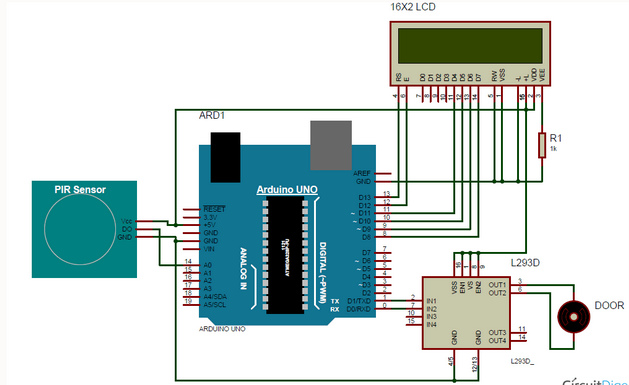
\includegraphics[scale = 0.5 ]{./figs/circuit.png}
\end{figure}

\subsection{Detailed study of each component}
\subsubsection{Arduino UNO}
The core component of the system, responsible for processing sensor inputs and controlling the door-opening mechanism. \\
The connections made from it are as shown below:
\begin{table}[H]
    \centering
    \begin{tabular}{|c|c|c|c|c|}
    \hline
    \textbf{Section} & \textbf{Pins in ARD} & \textbf{Other Device} & \textbf{Pins in other device} & \textbf{Pin number (if any)} \\
    \hline
    \multirow{3}{*}{Power} & \multirow{3}{*}{+5V} & PIR & $V_{CC}$ & - \\
    \cline{3-5}
    & & LCD & +L, VDD & 15, 2 \\
    \cline{3-5}
    & & L293D & $V_{CC1}, V_{CC2}, $EN1, EN2 & 16, 8, 1, 9 \\
    \hline
    \multirow{2}{*}{GND} & \multirow{2}{*}{GND} & PIR & GND & - \\
    \cline{3-5}
    & & L293D & GND & 4 and 12 OR 5 and 13 \\
    \cline{3-5}
    & & LCD & RW, $V_{SS}$, -L, $V_{EE}$ & 5, 1, 16, 3 \\
    \hline
    Analog & A0 & PIR & Digital output & - \\
    \hline
    \multirow{3}{*}{Digital} & D13, D12, D11 TO D8 & LCD & RS, Enable, D4 TO D7 & 4, 6, 11 TO 14 \\
    \cline{2-5}
    & D1/TXD, D0/RXD & L293D & IN1, IN2 & 2,7 \\
    \hline
    \end{tabular}
\end{table}

Pin diagram of ARD is as shown below:
\begin{figure}[H]
\centering
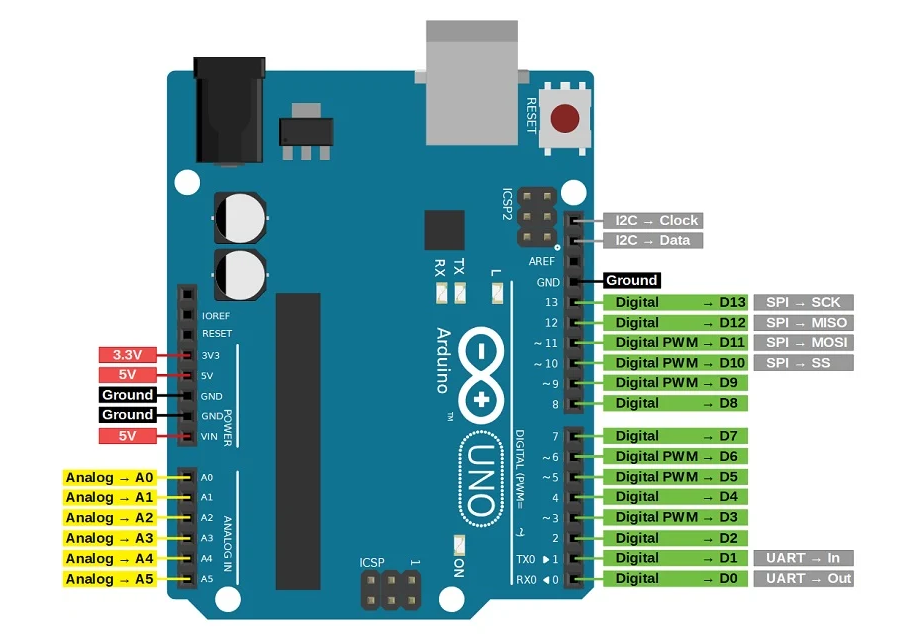
\includegraphics[scale = 0.3 ]{./figs/ardpindia.png}
\end{figure}
\textbf{CONNECTIONS:\\}
The Arduino consists of three main sections: Power, Analog, and Digital.
\begin{enumerate}
\item \textbf{Power Section}
\begin{itemize}
\item It includes the reset pin (not utilized here), voltage pin, ground, and AREF (analog reference, not used here).
\item The 5V pin is connected to the power pins of the PIR sensor, LCD, and motor driver. The ground pin is connected to the respective grounds of these components. Other connections from this section are outlined below.
\item The backlight connections of the LCD, denoted as +L and -L, are connected to +5V and ground respectively. These connections power the backlight to illuminate the LCD panel.
\item The RW (read/write) pin of the LCD is permanently connected to ground on the Arduino, allowing write operations (sending commands).
\item Another connection involves linking the ground of the Arduino to $V_{EE}$ of the LCD to control the display contrast. A 1k resistor is included in this connection to optimize contrast.
\item Additional connections to the motor driver IC (L293D) include the enable pins, ensuring the motor driver remains enabled whenever the Arduino is powered on. This enables motor power whenever the PIR sensor outputs 1.
\end{itemize}

\item \textbf{Analog Section} \\
The only connection made in this section is to the PIR sensor, with its digital output connected to the A0 pin of the Arduino. This connection allows the Arduino to receive and process analog signals from the sensor.

\item \textbf{Digital Section} \\
These connections can be categorized into three groups:
\begin{itemize}
\item D13 and D12 of the Arduino are connected to RS and Enable pins of the LCD respectively. RS determines whether incoming data is interpreted as command or character data for display.
\item Connections from D11 to D8 of the Arduino are respectively linked to D4 to D7 of the LCD for later use.
\item Finally, D1/TXD (transmitting) and D0/RXD (receiving) of the Arduino are connected to IN1 and IN2 of the Motor Driver respectively. These connections control the motor direction based on the logic levels of IN1 and IN2.
\end{itemize}
\end{enumerate}
\textbf{TESTING:}
\begin{enumerate}
\item Begin by connecting the Arduino board to a laptop.
\item Open the Arduino IDE and test the board using the example code for blinking an LED.
\item Verify that the LED blinks as expected, indicating proper functionality of the Arduino board.
\end{enumerate}



\subsubsection{16X2 LCD}
In an automatic door opening system, a 16x2 LCD (Liquid Crystal Display) can be used as a user interface to provide feedback, display status information, and enable user interaction. \\
The connections made from it are as shown below:


\begin{table}[H]
\centering
  \begin{tabular}{|c|c|c|c|}
    \hline
    \textbf{Pins in PIR} & \textbf{Other Device} & \textbf{Pins in other device} & \textbf{Pin number (if any)} \\
    \hline
     $V_{SS}$, RW, -L, $V_{EE}$ & ARD & GND & - \\
    \hline
    $V_{DD}$, +L & ARD & +5V & -  \\
    \hline
    RS, E, D4 TO D7 & ARD & D13 TO D8 & - \\
    \hline
  \end{tabular}
\end{table}

Pin diagram of LCD is as shown below:
\begin{figure}[H]
\centering
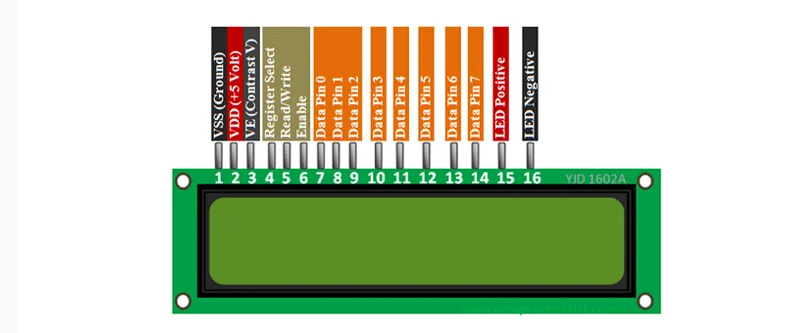
\includegraphics[scale = 0.4]{./figs/lcdpindia.png}
\end{figure}
\textbf{CONNECTIONS:\\}
All connections to this device are established through the Arduino board, as detailed in the preceding section.



\subsubsection{PIR Sensor}
In an automatic door opening system project, a PIR (Passive Infrared) sensor plays a crucial role in detecting motion and triggering the door's opening mechanism. \\
The connections made from it are as shown below:

\begin{table}[H]
    \centering
    \begin{tabular}{|c|c|c|c|}
    \hline
    \textbf{Pins in PIR} & \textbf{Other Device} & \textbf{Pins in other device} & \textbf{Pin number (if any)} \\
    \hline
    \multirow{3}{*}{Power Supply ($V_{CC}$)} & ARD & +5V (power) & - \\
    \cline{2-4}
    & LED & +L, VDD & 15, 2 \\
    \cline{2-4}
    & L293D & $V_{SS}$, EN1, $V_S$, EN2 & 16, 1, 9, 8 \\
    \hline
    Digital Output (DO) & ARD & Analog Output (analog) & - \\
    \hline
    \multirow{2}{*}{Ground (GND)} & ARD & GND (power) & - \\
    \cline{2-4}
     & L293D & GND & 4 and 12 OR 5 and 13 \\
    \hline
    \end{tabular}
\end{table}



Pin diagram of PIR Sensor is as shown below:
\begin{figure}[H]
\centering
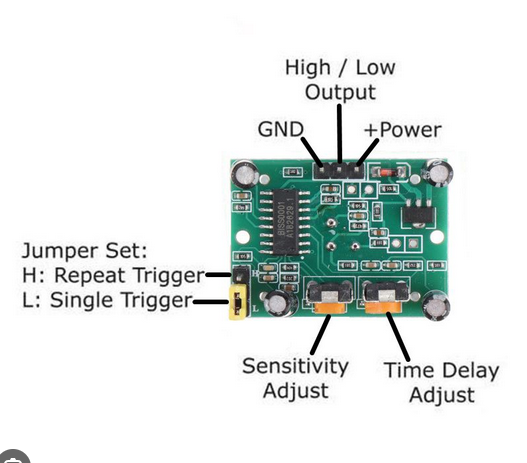
\includegraphics[scale = 0.5]{./figs/pirpindia.png}
\end{figure}
\textbf{CONNECTIONS:\\}
All connections to this device are established through the Arduino board, as detailed in the preceding section. \\
\textbf{TESTING}
\begin{enumerate}
\item Connect the circuit as shown below. \\
\begin{figure}[H]
\centering
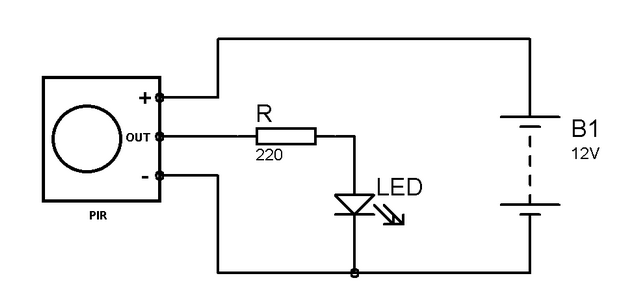
\includegraphics[scale = 0.5]{./figs/pirtest.png}
\end{figure}
\item Place your hand near the sensor. It passes the test if LED glows.
\end{enumerate}



\subsubsection{Motor Driver: L293D (IC)}
In an automatic door opening system project, the L293D motor driver IC is used to control the movement of the door mechanism, providing the necessary power and direction control for the motor.  \\
Pin diagram of L293D is as shown below:
\begin{figure}[H]
\centering
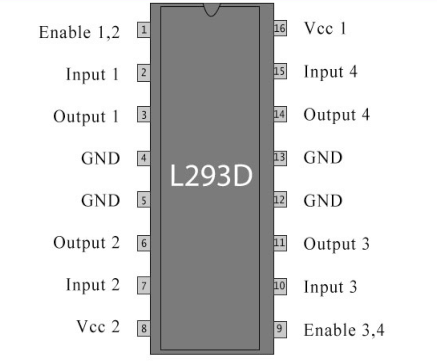
\includegraphics[scale = 0.5]{./figs/icpindia.png}
\end{figure}
\textbf{CONNECTIONS:}
\begin{enumerate}
\item Most of the connections to this device are facilitated by the Arduino (ARD), as previously outlined.
\item Additionally, OUT1 and OUT2 from the Arduino are connected to the motor, enabling its movement.
\end{enumerate}

\subsection{Programming}
\subsubsection{Code}
\input{./codes/code.cpp}
\subsubsection{Explaination}
\begin{enumerate}
    \item \textbf{Library Inclusion}:
        \begin{itemize}
            \item The code includes the necessary libraries, such as LiquidCrystal.h, to interface with the LCD display.
        \end{itemize}
        
    \item \textbf{Pin Definition}:
        \begin{itemize}
            \item Pin assignments for the LCD, PIR sensor, and gate motor are defined using preprocessor directives.
        \end{itemize}
        
    \item \textbf{Setup Function}:
        \begin{itemize}
            \item The setup function initializes the LCD and configures pins for input and output.
            \item Initial messages are displayed on the LCD to indicate system readiness.
        \end{itemize}
        
    \item \textbf{Loop Function}:
        \begin{itemize}
            \item The loop function continuously monitors the PIR sensor for motion detection.
            \item Upon detecting motion, the system activates the gate motor to open the gate and displays relevant messages on the LCD.
            \item After a delay, the gate motor is stopped temporarily before closing the gate.
            \item The system repeats this process as long as motion is detected.
        \end{itemize}
\end{enumerate}








\subsection{Sequential Mechanism}

The automatic door opening system operates through the following sequence:

\begin{enumerate}
    \item \textbf{Initialization}:
        \begin{itemize}
            \item The system powers on, initializing all components.
            \item The LCD display shows an initial message indicating system readiness, such as "Automatic Door Opener."
        \end{itemize}
        
    \item \textbf{Monitoring for Motion}:
        \begin{itemize}
            \item The PIR sensor continuously monitors its surroundings for motion.
        \end{itemize}
        
    \item \textbf{Detection of Motion}:
        \begin{itemize}
            \item Upon detecting motion, the PIR sensor sends a signal to the Arduino Uno.
        \end{itemize}
        
    \item \textbf{Decision Making}:
        \begin{itemize}
            \item The Arduino Uno processes the signal from the PIR sensor to determine if someone is approaching the door.
            \item If motion is detected, the Arduino Uno decides to initiate the door-opening sequence.
        \end{itemize}
        
    \item \textbf{Initiating Door Opening}:
        \begin{itemize}
            \item The Arduino Uno sends signals to the motor driver to activate the door-opening motor.
        \end{itemize}
        
    \item \textbf{Door Opening}:
        \begin{itemize}
            \item The motor rotates, smoothly opening the door.
            \item The LCD display shows a message indicating that the door is opening.
        \end{itemize}
        
    \item \textbf{Monitoring Door Position}:
        \begin{itemize}
            \item The system continuously monitors the position of the door to ensure it reaches the fully open position.
        \end{itemize}
        
    \item \textbf{Door Fully Opened}:
        \begin{itemize}
            \item Once the door reaches the fully open position, the motor stops, and the Arduino Uno receives confirmation.
        \end{itemize}
        
    \item \textbf{Waiting for Motion to Cease}:
        \begin{itemize}
            \item If no motion is detected for a predefined period, the system waits for motion to cease.
        \end{itemize}
        
    \item \textbf{Detection of No Motion}:
        \begin{itemize}
            \item If no motion is detected for the predefined period, the PIR sensor sends a signal to the Arduino Uno indicating the absence of motion.
        \end{itemize}
        
    \item \textbf{Closing the Door}:
        \begin{itemize}
            \item Upon receiving the signal indicating the absence of motion, the Arduino Uno initiates the door-closing sequence.
            \item It sends signals to the motor driver to activate the motor in the reverse direction, causing the door to close.
        \end{itemize}
        
    \item \textbf{Door Closing}:
        \begin{itemize}
            \item The motor rotates in the reverse direction, closing the door.
            \item The LCD display shows a message indicating that the door is closing.
        \end{itemize}
        
    \item \textbf{Monitoring Door Position}:
        \begin{itemize}
            \item The system continuously monitors the position of the door to ensure it reaches the fully closed position.
        \end{itemize}
        
    \item \textbf{Door Fully Closed}:
        \begin{itemize}
            \item Once the door reaches the fully closed position, the motor stops, and the Arduino Uno receives confirmation.
        \end{itemize}
        
    \item \textbf{Idle State}:
        \begin{itemize}
            \item The system returns to an idle state, ready to detect motion and initiate the door-opening sequence again when necessary.
        \end{itemize}
\end{enumerate}

\textbf{NOTE:} We haven't connected a door in here. So the clockwise and anticlockwise rotation of door shows the opening and closing of door. 





\section{Results}
[Present the data collected during the experiment. This may include tables, graphs, or other visual representations of the data. Provide any calculations performed and describe any trends or patterns observed in the data.]

\section{Discussion}
[Interpret the results obtained and explain their significance. Compare the results with the expected outcomes based on the theory or hypothesis. Discuss any sources of error or limitations of the experiment. Address any unexpected results and propose possible explanations.]

\section{Conclusion}
[Summarize the key findings of the experiment. Restate the main conclusions drawn from the results. Discuss any implications of the findings and suggest areas for future research or improvements to the experiment.]

\section*{References}
[List any sources cited in the report, including textbooks, journal articles, or other relevant materials.]

\section*{Appendices}
[Include any supplementary information such as raw data, calculations, or additional figures that support the findings of the experiment.]

\end{document}

